%!TEX root = ./main.tex

\chapter{Final results, discussion and conclusion} % (fold)
\label{sec:final_results_discussion_and_conclusion}

\section{Test environment} % (fold)
\label{sec:test_environment}

To test and investigate our results three test environments have been used, as shown in Table~\ref{sec:test_environment}. They all have different properties that are used to test different aspects of our algorithms. Test environment 3 has a normal windows setup, with a graphics card that is used for both display rendering and CUDA computation. On the other hand, test environment 1, uses the same hardware, but is setup with a dedicated GPU\@. CUDA computations done on a environment without a dedicated GPU, is forced to split the resources with the running OS, which implies some restrictive properties. For instance, it is normal for an OS to kill long running processes. On windows the normal timeout is around $30$ seconds. To get around this restriction some editing in regedit is necessary.

The last environment, number 2, is build on a amazon instance. This give us a way to test one a wither and a more powerful computer. In our case, as our specific application needs a high number of points, the biggest  and discussionadvantage was huge memory capacity on the amazon system. Increased number of CUDA cores also made it possible to test performance ratios and different variants of resource distributions.

\begin{table}[ht]
\centering
    \begin{tabular}{|l|l|l|l|}
        \hline
        \textbf{Test envoronment} & \textbf{1}         & \textbf{2}       & \textbf{3}\\ \hline
        \textbf{OS}               & Ubuntu 14.04       & Ubuntu 12.04     & Windows 7  \\ \hline
        \textbf{OS type}          & x64                & x64              & x64     \\ \hline
        \textbf{Kernel}           & 3.13.0-24-generic  & 3.2.0-58-virtual & Windows 7      \\ \hline
        \textbf{CPU}              & i7-2600K           & E5-2670          & i7-2600K       \\ \hline
        \textbf{CPU memory}       & 7.8 Gb             & 16 Gb            & 7.8 Gb \\ \hline
        \textbf{GPU}              & GeForce GTX 560 Ti & NVIDIA GRID K520 & GeForce GTX 560 Ti      \\ \hline
        \textbf{GPU memory}       & 1024 Mb            & 4095 MB          & 1024 Mb      \\ \hline
        \textbf{Dedicated GPU}    & Yes                & Yes              & No       \\ \hline
        \textbf{CUDA cores}       & 384                & 1536             & 384       \\ \hline
        \textbf{CUDA capability}  & 2.1                & 3.0              & 2.1       \\ \hline
        \textbf{CUDA driver}      & 5.5                & 5.5              & 5.5       \\ \hline
        \textbf{CUDA runtime}     & 5.5                & 5.5              & 5.5       \\ \hline
    \end{tabular}
    \caption{Tabulated information about the three test environments.}
    \label{tbl:test_envoronments}
\end{table}

All tests was run multiple times and averaged, to get more accurate results. It should also be noted that it is common practice to warm up the GPU before any test. Reason is that it may take as long time for the CUDA runtime to create a CUDA context, as launching the kernel itself.
% section test_envorinment (end)

\section{Final results and discussion} % (fold)
\label{sec:final_results_and_discusstion}

During the development of our algorithms, we have presented many intermediate results, in order to argument for the design and implementation choices made. In this section, we will present our final results for the GPU parallelized brute force, GPU parallelized and CPU parallelized k-d tree based kNN algorithm.

The different research questions stated during development of our algorithms are revisited, and answered are given, based on the presented results. 

\subsection{Solving the kNN problem} % (fold)
\label{sub:solving_the_knn_problem}

In Section~\ref{sec:brute_force_garcia} we started off our quest for a faster kNN search, by investigating a possible brute-force algorithm, pioneered by Garcia et.al. The following research question was asked. RQ~\ref{rq:brute_force_performance}, can high performance be achieved by a parallel brute force kNN algorithm on large point clouds.

In order to discuss this question, we have to clarify what we consider to be high performance in this context. The work of Garcia et.al. contains the fastest brute force algorithm, for solving the kNN problem, we have found in current literature. We would therefore consider a kNN algorithm to have high performance, if it is able to solve the kNN problem for point cloud data, in the 3D format specified by TSI, at comparable speeds to the algorithm developed by Garcia et.al. 

Although the algorithm developed by Garcia et.al. is the fastest brute force algorithm we have managed to find, this is not as a high benchmark as it might initially seem. The algorithm developed by Garcia et.al. is optimized for solving the kNN problem for a more general version of the kNN problem than required by TSI. Where we are only concerned with solving the kNN problem for three dimensions, Garcia's algorithm will solve problems stated in any dimension. Given that we solve a more restricted version of the kNN problem, any less than comparable speeds to the implementation made by Garcia et.al. could not be considered to be of high performance in our eyes.

\begin{figure}[ht!]
    \centering
    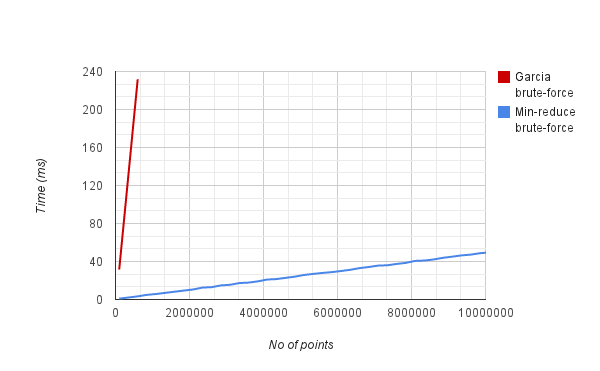
\includegraphics[width=120mm]{../gfx/fin-garcia-vs-min-reduce.png}
    \caption{Comparison of brute-force algorithm developed by Garcia et.al. and min-reduce based brute-force algorithm developed in this thesis. $k$ is fixed at 10 and $m$ is increasing.}
    \label{fig:fin-garcia-vs-min-reduce}
\end{figure}

In Section~\ref{sub:continuing_on_garcia_s_path}, we discussed Figure~\ref{fig:brute_force}. As a reminder, part of this figure is presented as Figure~\ref{fig:fin-garcia-vs-min-reduce}, which shows the result of a comparison between the brute force algorithm developed by Garcia et.al. and our min-reduce brute-force algorithm developed in Section~\ref{sub:continuing_on_garcia_s_path}. The test is performed with a low value for $k=10$, and focuses on performance for large values of number of points, $m$. In this test, our min-reduce brute-algorithm is shown to be almost $70$ times faster than the algorithm developed by Garcia et.al. In addition, it is capable of solving the kNN problem for much larger values of $m$.

We therefore conclude that RQ~\ref{rq:brute_force_performance} can be answered with yes. High performance can be achieved with a brute-force based algorithm.

In Section~\ref{sec:brute_force_garcia} we introduced the k-d tree, a data-structure with a known \BigO{log(m)} nearest neighbor query algorithm. We therefore presented RQ~\ref{rq:serial-kd-tree}: It is possible to use a k-d tree to increase the performance of kNN queries, compared to a parallel brute force solution? We try to answer this question in Figure~\ref{fig:final-knn-kd-vs-bf}.

\begin{figure}[ht!]
    \centering
    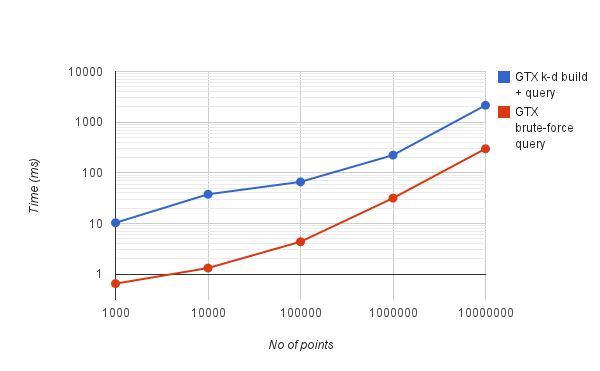
\includegraphics[width=120mm]{../gfx/final-knn-kd-vs-bf.png}
    \caption{Comparison of min-reduce brute-force and k-d tree based algorithms for solving the kNN problem for $k=100$ and increasing $m$.}
    \label{fig:final-knn-kd-vs-bf}
\end{figure}

The graph compares the runtime of the k-d tree build and query algorithms developed in Section~\ref{sec:development_of_a_parallel_k_d_search_algorithm} with the min-reduce brute-force algorithm. All test data is generated using test environment 1 \ref{tbl:test_envoronments}.

Figure~\ref{fig:final-var-knn-kd-vs-bf} compares the same two algorithms, but for a fixed value of $m$, and increasing value of $k$. This test is also performed using test environment 1 \ref{tbl:test_envoronments}.

\begin{figure}[ht!]
    \centering
    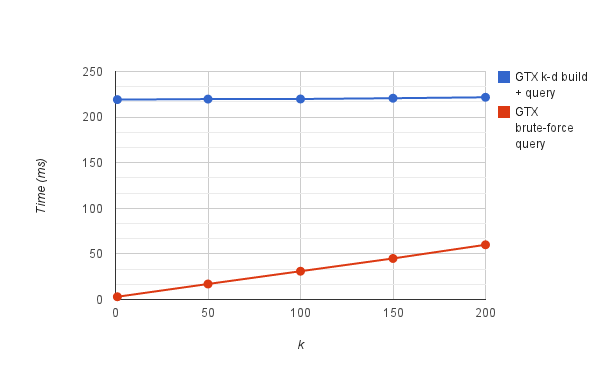
\includegraphics[width=120mm]{../gfx/final-var-knn-kd-vs-bf.png}
    \caption{Comparison of min-reduce brute-force and k-d tree based algorithms for solving the kNN problem for $m=1e6$ and increasing $k\le200$.}
    \label{fig:final-var-knn-kd-vs-bf}
\end{figure}

Both Figure~\ref{fig:final-knn-kd-vs-bf} and \ref{fig:final-var-knn-kd-vs-bf} shows that this algorithm is slower than a brute force approach. In order to solve the kNN problem, the k-d tree based solution first has to construct the k-d tree, then query for the closest points. Given that our previous calculation shows that the time complexity of the k-d tree build algorithm is larger than the time-complexity for the brute-force algorithm, this result should come as no surprise. Constructing the k-d data-structure for a single query is simply a waste of resources, if just one kNN query is to be performed.
% subsection solving_the_knn_problem (end)

\subsection{Solving the All-kNN problem} % (fold)
\label{sub:solving_the_all_knn_problem}

We have seen that performance of k-d search is not good enough 

RQ~\ref{rq:brute_force_Q-kNN} Can a parallel brute force kNN algorithm be fast enough to solve the All-kNN problem within reasonable time?

RQ~\ref{rq:serial-kd-tree-all-knn} It is possible to use a k-d tree to increase the performance of All-kNN queries, compared to a parallel brute force solution?

\begin{figure}[ht!]
    \centering
    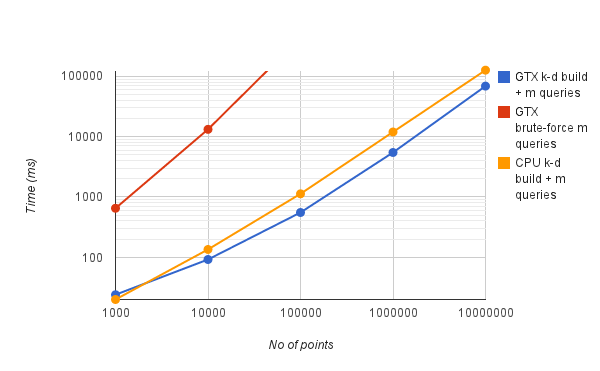
\includegraphics[width=120mm]{../gfx/final-all-knn-gpu-vs-cpu-vs-bf.png}
    \caption{Timing results for varying values of k with GPU parallelized algorithm.}
    \label{fig:final-all-knn-gpu-vs-cpu-vs-bf}
\end{figure}

\begin{figure}[ht
    \centering
    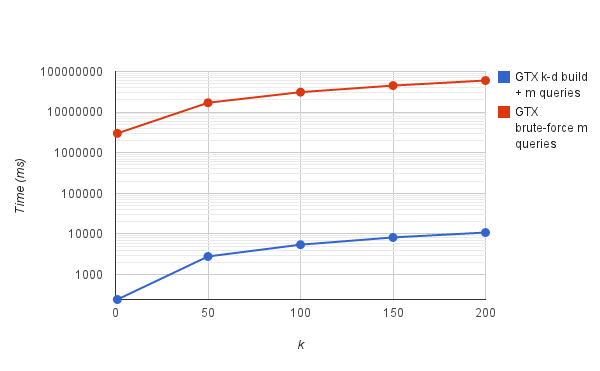
\includegraphics[width=120mm]{../gfx/final-var-all-knn-kd-vs-bf.png}
    \caption{Timing results for varying values of k with GPU parallelized algorithm.}

    The different research questions stated during development of our algorithms are revisited, and answerd
    \label{fig:final-var-all-knn-kd-vs-bf}
\end{figure}

Relation to solving the TSI problem. Something about solving the All-kNN problem is most related to this, bla bla.

Maybe a final graph with All-kNN, k = 100 for very large values of m? Just some data points?
% subsection solving_the_all_knn_problem (end)

\subsection{Parallelization performance increase} % (fold)
\label{sub:parallelization_performance_increase}
 Continuing on our quest for a fast kNN search, a parallelization of the k-d tree build was introduced with RQ~\ref{rq:parallel_build}, in Section~\ref{sec:development_of_a_parallel_k_d_tree_build_algorithm}.

\textbf{RQ~\ref{rq:parallel_build}.} \emph{It is possible to parallelize the k-d tree build algorithm, in such a way that it gives a significant speed improvement compared to the serial algorithm.}

The resource question is based around the complex nature of the k-d tree build, and the uncertainty of a acceptable parallel speedup. This question was investigated though implementation prototypes, together with a thorough discussion about the parallelization strategy and the intermediate results. 

\begin{figure}[ht!]
    \centering
    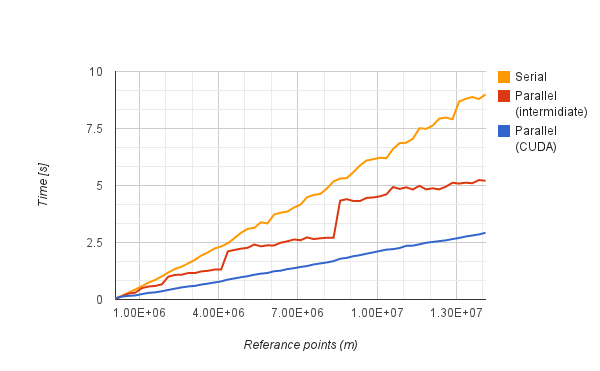
\includegraphics[width=120mm]{../gfx/final_tree_build.png}
    \caption{Comparison between serial and parallel k-d tree build performance.}
    \label{fig:final_tree_build}
\end{figure}

Figure~\ref{fig:final_tree_build} tries to answer RQ~\ref{rq:parallel_build}, by comparing the serial and parallel k-d tree build implementation. Both graphs follows the same trend, which correlates with the shared time complexity of \BigO{m\ log(m)}. We see that the impact of the parallel overhead is decreasing as the problem size increase, and the profit of multiple cores is getting more and more be dominant. Resulting in a faster parallel implementation.

To get a better picture of the parallel improvement, it is natural to talk about parallel speedup. Figure~\ref{fig:final_tree_build_speedup} shows how the parallel speedup develops, as the problem size increase. Here we see that the speedup starts below $1$, indicating that the serial version is faster then the parallel version, but from Figure~\ref{fig:final_tree_build} one can see that the time to build such small k-d trees is almost negligible. As the problem size increase, the trend quickly changes, until the speedup flattens out. The speedup increases as the problem size allows utilization of more and more threads, until the limit is reached, and the curve flattens out into a lower gradient.      

\begin{figure}[ht!]
    \centering
    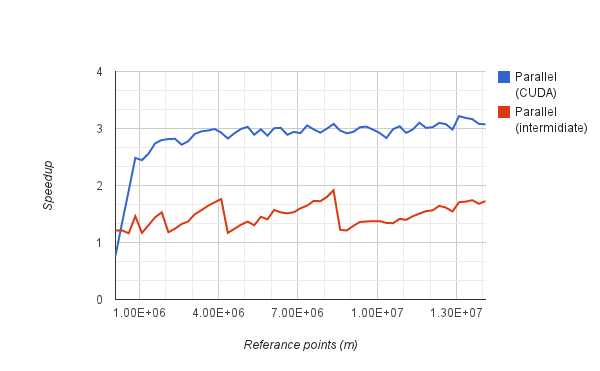
\includegraphics[width=120mm]{../gfx/final_tree_build_speedup.png}
    \caption{Parallel speedup for the k-d tree implementation for varying values of $m$.}
    \label{fig:final_tree_build_speedup}
\end{figure}

With the complex nature if a k-d tree build process, a speedup of three is acceptable, and we categorize it as a significant improvement, which answer RQ~\ref{rq:parallel_build}. 


RQ~\ref{rq:parallel_query} proposed the next topic of our quest, namely the parallelization of the All-kNN query. 

\textbf{RQ~\ref{rq:parallel_query}.} \emph{It is possible to parallelize the All-kNN query algorithm, in such a way that it gives a significant speed improvement compared to the serial algorithm.}

\begin{figure}[ht!]
    \centering
    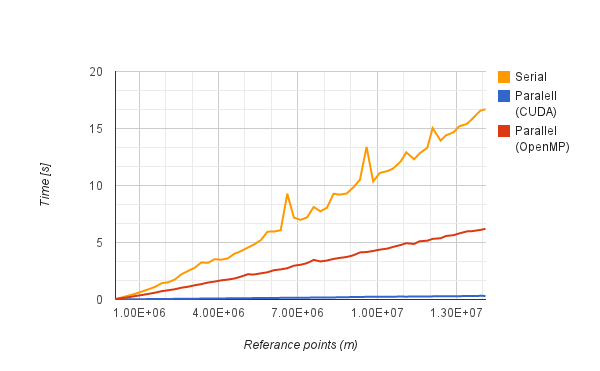
\includegraphics[width=120mm]{../gfx/final_kd_search.png}
    \caption{Comparison between serial and parallel All-kNN query performance.}
    \label{fig:final_kd_search}
\end{figure}

Figure~\ref{fig:final_kd_search} visualize the results from the two different parallel All-kNN query implementations, CUDA and OpenMP, compared to the serial version. The linear trend, also found in the k-d tree build algorithm, is not surprising, as the time complexity for all algorithms are \BigO{m\ log(m)}. The parallel improvement is only shown in the gradient these slopes have, which is reasonable, because the work is only divided amongst more cores. In both OpenMp and CUDA the parallel improvement is significant.

\begin{figure}[ht!]
    \centering
    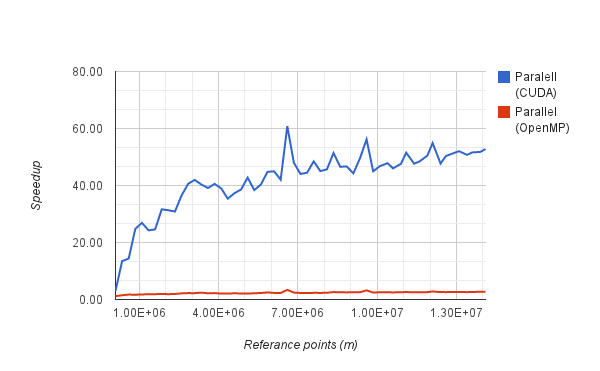
\includegraphics[width=120mm]{../gfx/final_kd_search_speedup.png}
    \caption{Parallel speedup comparison for the All-kNN query between the CUDA and OpenMP implementation.}
    \label{fig:final_kd_search_speedup}
\end{figure}

If we look at the parallel speedup, shown in Figure~\ref{fig:final_kd_search_speedup}, we can again conclude that the OpenMP version is outperformed by the CUDA implementation. The trend resembles what we saw in the k-d tree build parallelization, only this time the speedup goes towards $50$ in the CUDA version. This correlations perfectly with the discussion, in Section~\ref{sub:parallelization_strategy}, about the parallelization strategy and how easily the work could be partitioned.      

An interesting note is that this speedup is lower then in both our and Garcia's\cite{Garcia2008} brute force implementations, which implies that speedup don't equal a fast implementations. It only implies a good parallel performance increase, compared to the serial algorithmic in use.

This answers RQ~\ref{rq:serial-kd-tree}, and we conclude that our All-kNN query has a significant parallel improvement.
% subsubsection parallelization_of_the_k_d_tree_build (end)



% subsection parallelization_performance_increase (end)


During the development of our algorithms, we have presented many intermediate results, in order to argument for the design and implementation choices made. In this section, we will present our final results for the GPU parallelized brute force, GPU parallelized and CPU parallelized k-d tree based kNN algorithm.

We wanted to test the performance of our algorithms as closely as possible to the TSI point cloud use-case. This meant exploring the performance of the algorithms for solving the All-kNN problem for point clouds in the order of magnitude $1e7$ and values of $k<=100$. As well as exploring the requirements stated by TSI, we wanted the test set to be able to run within reasonable time, since we wanted to be able to run the same tests for every major update to our implementation. To do this two test cases where set up.

Test case one, is concerned with exploring the performance of the algorithm, when solving the All-kNN problem for a large number of points $1e7<=n<=2e7$. We initially wanted to perform this test for several test series with $k$ varying from one to a hundred. Unfortunately, due to the size of $n$, this test ended up consuming all our system memory (RAM) for higher values of $k$, as well as being a very time consuming test set to run. To get around this limitation, we choose to restrict $k$ to one in this test set, just focusing on the performance related to scaling $n$.

In order to explore the performance of the different algorithms when scaling $k$, we constructed a second set of tests. In test case two, several test-runs on point clouds ranging from $1e7<=n<=2e7$ is performed. Each with a different value for $1<=k<=100$, but instead for solving the All-kNN problem, we are solving the Q-kNN problem for $Q=10^6$. This way we where able to test the algorithm for the same range of $n$. Since the difference between the All-kNN problem and the Q-kNN problem is only concerned with the number of consecutive queries performed, the relative speed difference arising from changing the value of $k$ is the same.

All tests where performed on synthetic data, with a set of points uniformly distributed in a unit cube in the first octant.

Let us first look at the results for the GPU parallelized and CPU parallelized k-d tree based algorithm.

Figure \ref{fig:v17-gtx-560} shows the performance of the GPU parallelized k-d tree based build and query algorithm. Since the query time and build time is shown as individual graphs, the total time for solving the All-kNN problem for a given problem size is the sum of the build and the query time.

\begin{figure}[ht!]
    \centering
    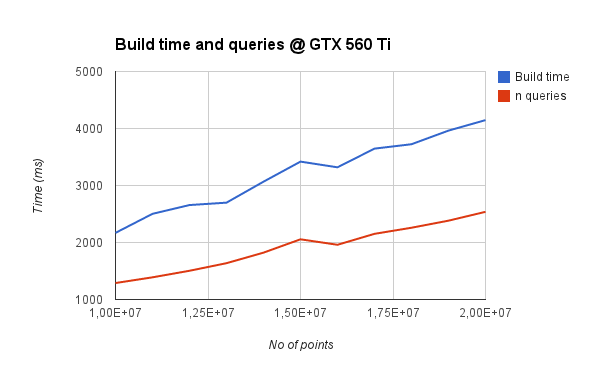
\includegraphics[width=120mm]{../gfx/v17-gtx-560.png}
    \caption{Timing results for k-d tree build and n query with k equal to one. Test performed on GTX 560.}
    \label{fig:v17-gtx-560}
\end{figure}

As expected, both algorithms scale quite linearly, with some deviation, especially around $n=1,5e7$. We do not consider this deviation to be of statistical significance, and is most probably due to test machine running other processes during the test. The correlation between the build results and the query results, is also most probably explained by the build and query timing data being gathered from the same run of the program.

In the final version of the GPU parallelized versions of the k-d tree algorithms we note that optimization of the original algorithm has managed to bring the query time for the All-kNN problem below the time needed for building the tree. We are, in other word, able to solve the kNN problem for all the points in the tree in about halve the time it takes to build the data structure. This is a big improvement compared to the initial parallel implementation, which ran substantially slower than the build algorithm.

The results show that our implementation is able to solve the All-kNN problem, with $k=1$, for a point cloud of 20 million in about $6,7$ seconds.

In figure \ref{fig:v17-gpu-variable-k} we sew how increasing $k$ affects our run time.

\begin{figure}[ht!]
    \centering
    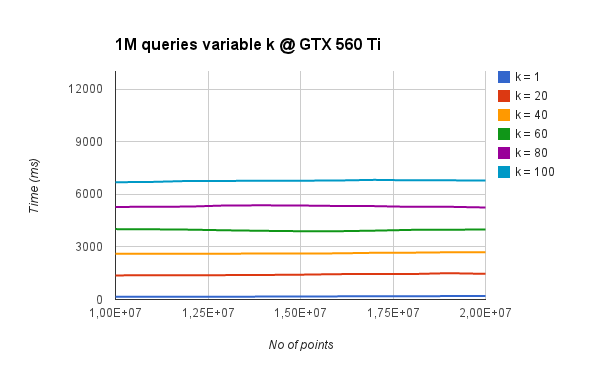
\includegraphics[width=120mm]{../gfx/v17-gpu-variable-k.png}
    \caption{Timing results for varying values of k with GPU parallelized algorithm.}
    \label{fig:v17-gpu-variable-k}
\end{figure}

The results seem to indicate that increasing $k$ adds a constant factor penalty to the runtime of the query algorithm. For each increment of $20$ in $k$, we see a corresponding increase in the runtime of about $1200$ to $1400$ ms. Although the runtime increase is constant, it is quite significant, dominating the increase in runtime caused by increasing the number of points. If we e.g. compare the test series for $k=20$ and $k=40$, the runtime for $k=20$ and $k=40$ increases with just about $90$ ms when $n$ is increased from $1e7$ to $2e7$. In comparison, the average runtime difference between the series is about $1200$ ms. In both cases both $k$ and $n$ is doubled, so despite the large difference in absolute value, this supports the assessment that scaling $k$ is a more expensive operation than scaling $n$ for this algorithm. This nature is not optimal, but is still a good fit for the requirements stated by TSI.

% Remember to include information about the AWS hardware setup
In order to investigate the performance of the GPU parallelized k-d tree based algorithm on hardware designed for GPGPU applications, test case one where repeated on a rented GPGPU graphics card supplied by Amazon Web Service (AWS). The main difference between the AWS GPU and the GTX 560 Ti, is that the AWS GPU have more memory available on the GPU itself, 4Gb compared to 1Gb, as well as more parallel cores and threads. In addition, it is running system software, optimized for GPGPU applications. The additional GPU memory allowed us to run the All-kNN query for a larger number of points $1e7<=n<=1e8$. Figure \ref{fig:v17-aws} shows the results obtained.

\begin{figure}[ht!]
    \centering
    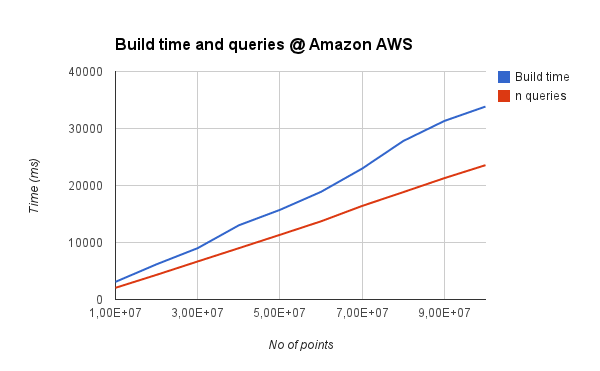
\includegraphics[width=120mm]{../gfx/v17-aws.png}
    \caption{Timing results for k-d tree build and n query with k equal to one. Test performed on Amazon web service.}
    \label{fig:v17-aws}
\end{figure}

The linear increase in runtime seem to be present in this graph as well, especially for the query algorithm. Comparing the runtime of the build and query algorithms, the query still take less time then the build, but the runtime is initially closer than in figure \ref{fig:v17-gtx-560}, and the gap widens when $n$ increases. This is a trend that was not initially present when testing on the GTX 560, and may have been caused by the smaller difference in $n$ used when testing on the GTX. In addition, and quite surprisingly, the AWS GPU is slower than the GTX 560 in solving All-kNN for $n=1e7$ and $n=2e7$. An interesting result, considering that the AWS GPU should supposedly be better suited to GPGPU applications.

The CPU parallelized version of the k-d tree based query algorithm was also subjected to both test cases. Figure \ref{fig:v17-gpu-vs-cpu} shows the runtime of the query algorithm in both the GPU and CPU parallelized version, subjected to test case one.

\begin{figure}[ht!]
    \centering
    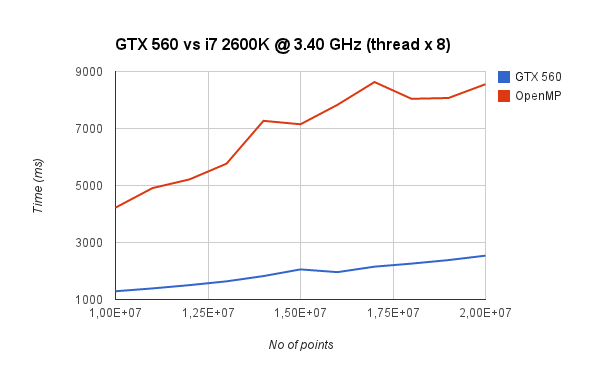
\includegraphics[width=120mm]{../gfx/v17-gpu-vs-cpu.png}
    \caption{Comparison of runtime for GPU (GTX 560) and CPU (OpenMP) parallelized k-d tree based n query.}
    \label{fig:v17-gpu-vs-cpu}
\end{figure}

Figure \ref{fig:v17-cpu-variable-k} shows how the CPU parallelized query performs when subjected to test case two.

\begin{figure}[ht!]
    \centering
    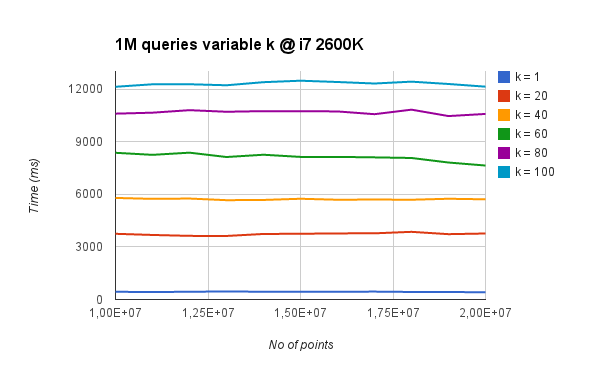
\includegraphics[width=120mm]{../gfx/v17-cpu-variable-k.png}
    \caption{Timing results for varying values of k with CPU parallelized algorithm.}
    \label{fig:v17-cpu-variable-k}
\end{figure}

In both figure \ref{fig:v17-gpu-vs-cpu} and figure \ref{fig:v17-cpu-variable-k} the CPU based parallelization is slower than the GPU based parallelization. This indicates, that for this algorithm, the benefit of having faster individual cores, and less overhead related to memory transfer on the CPU, is not enough to offset the drawback of the CPU has a lot fewer parallel cores than the GPU.

Let us now have a look at how the brute-force algorithm performs subjected to these tests. Due to the low performance of the brute-force algorithm on repeated queries, test case one and two had to be modified. In both cases, we are testing our implementation on the kNN problem, and multiplying the timing result with $n$ and $q$. This will still give us a good approximation of the actual run time, since the brute-force algorithm is just executed sequentially when solving All-kNN and Q-kNN problems. Figure \ref{fig:brute-force-query} shows the estimated timing results obtained by testing the brute-force algorithm this way.

\begin{figure}[ht!]
    \centering
    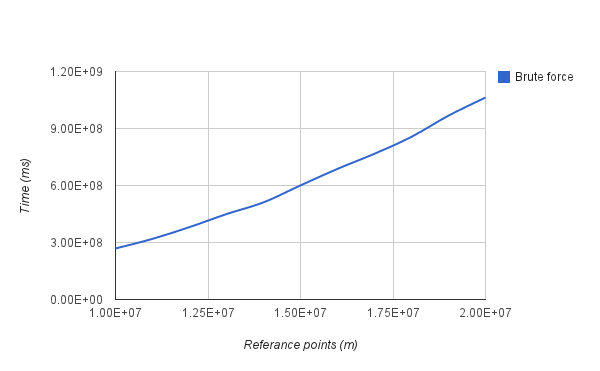
\includegraphics[width=120mm]{../gfx/brute-force-query.png}
    \caption{Timing results for brute force query with k equal to one. Test performed on GTX 560.}
    \label{fig:brute-force-query}
\end{figure}

The results from test case one confirms what our initial calculations indicated. The brute-force algorithm is very slow when applied to the All-kNN problem. Even solving All-kNN for the smallest point cloud $n=1e7$ would require approximately $2,7e8$ ms, or 75 hours.

Figure \ref{fig:brute-force-variable-k} show the performance of the brute force algorithm on test case two.

\begin{figure}[ht!]
    \centering
    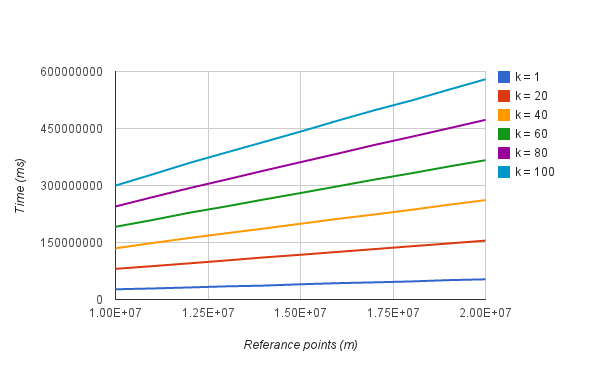
\includegraphics[width=120mm]{../gfx/brute-force-variable-k.png}
    \caption{Timing results for the brute force algorithm with varying values of k. Test performed on GTX 560.}
    \label{fig:brute-force-variable-k}
\end{figure}

Increasing the value for $k$ shows a trend similar in overall to the k-d tree based algorithm, but with overall slower results. Another difference is that increasing $k$ from 80 to 100 seems to give a lover penalty than increasing $k$ from 1 to 20.
% section final_results_and_discusstion (end)

\section{Conclusion} % (fold)
\label{sec:conclusion}

Fast algorithms have been made. The developed library of CUDA parallelized algorithms are significantly faster than comparable literature.

Brute force is good for single, non-repeated, kNN queries.

To solve All-kNN k-d trees is best. Big improvement over brute force approach.

All-kNN is even so fast that TSI goal can be achieved. This was not possible with conventional algorithms. 

In our work GPGPU has been a success, and should be explored for other problems as well.

Some reccomendations for further work.
% section conclusion (end)
